\makeatletter
\def\input@path{{headers/}}
\makeatother
\documentclass{beamer}

\usepackage{beamer_tom}
\usepackage{hyperref}
\graphicspath{{./images/}}


\institute{INRIA Saclay}
\author{Thomas Moreau}
\title{
    Benchopt:\\
    Benchmarking optimization Algorithms
}

\date{
    May 29, 2018
}

\setbeamertemplate{title page}[frame]
\def\extraLogo{}


\begin{document}

    \begin{frame}
        \titlepage
    %	\biblio{}
    \end{frame}

    \frame{
        \frametitle{Benchmarking algorithms in practice}

        Choosing the best algorithm to solve an optimization problem often depends on:\\[1em]
        \begin{minipage}{.8\textwidth}
            \begin{itemize}
                \item The data \keypoint{scale, conditionning}
                \item The objective parameters \keypoint{regularisation}
                \item The implementation \keypoint{complexity, language}
            \end{itemize}
        \end{minipage}

        \vskip2em
        An impartial selection requires a time consuming {\bf benchmark}!\\[1em]


        The goal of {\bf Benchopt} is to make this step as easy as possible.

    }

    \frame{
        \frametitle{Benchopt}

        % It can be installed through:\\[.5em]
        % {\centering  \code{pip install benchopt}\\[1em]}

        Doing a  benchmark for the $\ell_2$ regularized logistic regression with multiple solvers and datasets is now easy as calling:\\[1em]

        \begin{beamercolorbox}[
            shadow=true, wd=.96\textwidth, sep=.2em, rounded=true
        ]{title}
            \textcolor[rgb]{0,.3,.6}{
                \texttt{git clone https://github.com/benchopt/benchmark\_logreg\_l2}\\
                \texttt{benchopt run ./benchmark\_logreg\_l2}}
        \end{beamercolorbox}

        \vskip1.5em
        \includegraphics[width=.45\textwidth]{logreg_l2}
        \hskip3ex
        \includegraphics[width=.45\textwidth]{logreg_l2_1}
    }

    \frame{
        \frametitle{Benchopt}

        Benchopt can also compare the same algo in different languages.\\[1em]

        Here is an example comparing PGD in: Python; R; Julia.\\[1em]
        {\centering
        \vskip.5em
        \includegraphics[width=.65\textwidth]{lasso_3_languages}\\}
    }

    \frame{
        \frametitle{Benchmark: principle}

        A benchmark is a directory with:\\[.5em]
        \begin{itemize}
            \item An \code{objective.py} file with an \code{Objective},
            \item A directory \code{solvers} with one file per \code{Solver},
            \item A directory \code{datasets} with \code{Dataset} generators/fetchers.
        \end{itemize}
        \vskip1em
        Each of these objects can be parametrized.\\[2em]

        The \code{benchopt} client runs a cross product and generates a csv file + convergence plots like above.\\[.5em]
        We expose easy way to select the \code{objective/solver/dataset} you want to run.
    }

    \frame{
        \frametitle{Benchmarks}
        So far, we have implemented benchmarks for:\\[.5em]
        \begin{itemize}
            \item Least Square
            \item Non-Negative Least Square
            \item Lasso
            \item L1/L2 Regularized Logistic Regression
        \end{itemize}

        \vskip1em
        But feel free to join our effort to create reproducible benchmarks by adding new objectives/solvers/datasets!!!\\[1em]

        \includegraphics[width=.19\textwidth]{agramfort}
        \includegraphics[width=.19\textwidth]{jsalmon}
        \includegraphics[width=.19\textwidth]{mmassias}
        \includegraphics[width=.19\textwidth]{tomdlt}
        \includegraphics[width=.19\textwidth]{tommoral}
    }

    \frame{
        \frametitle{Benchopt}
        \centering
        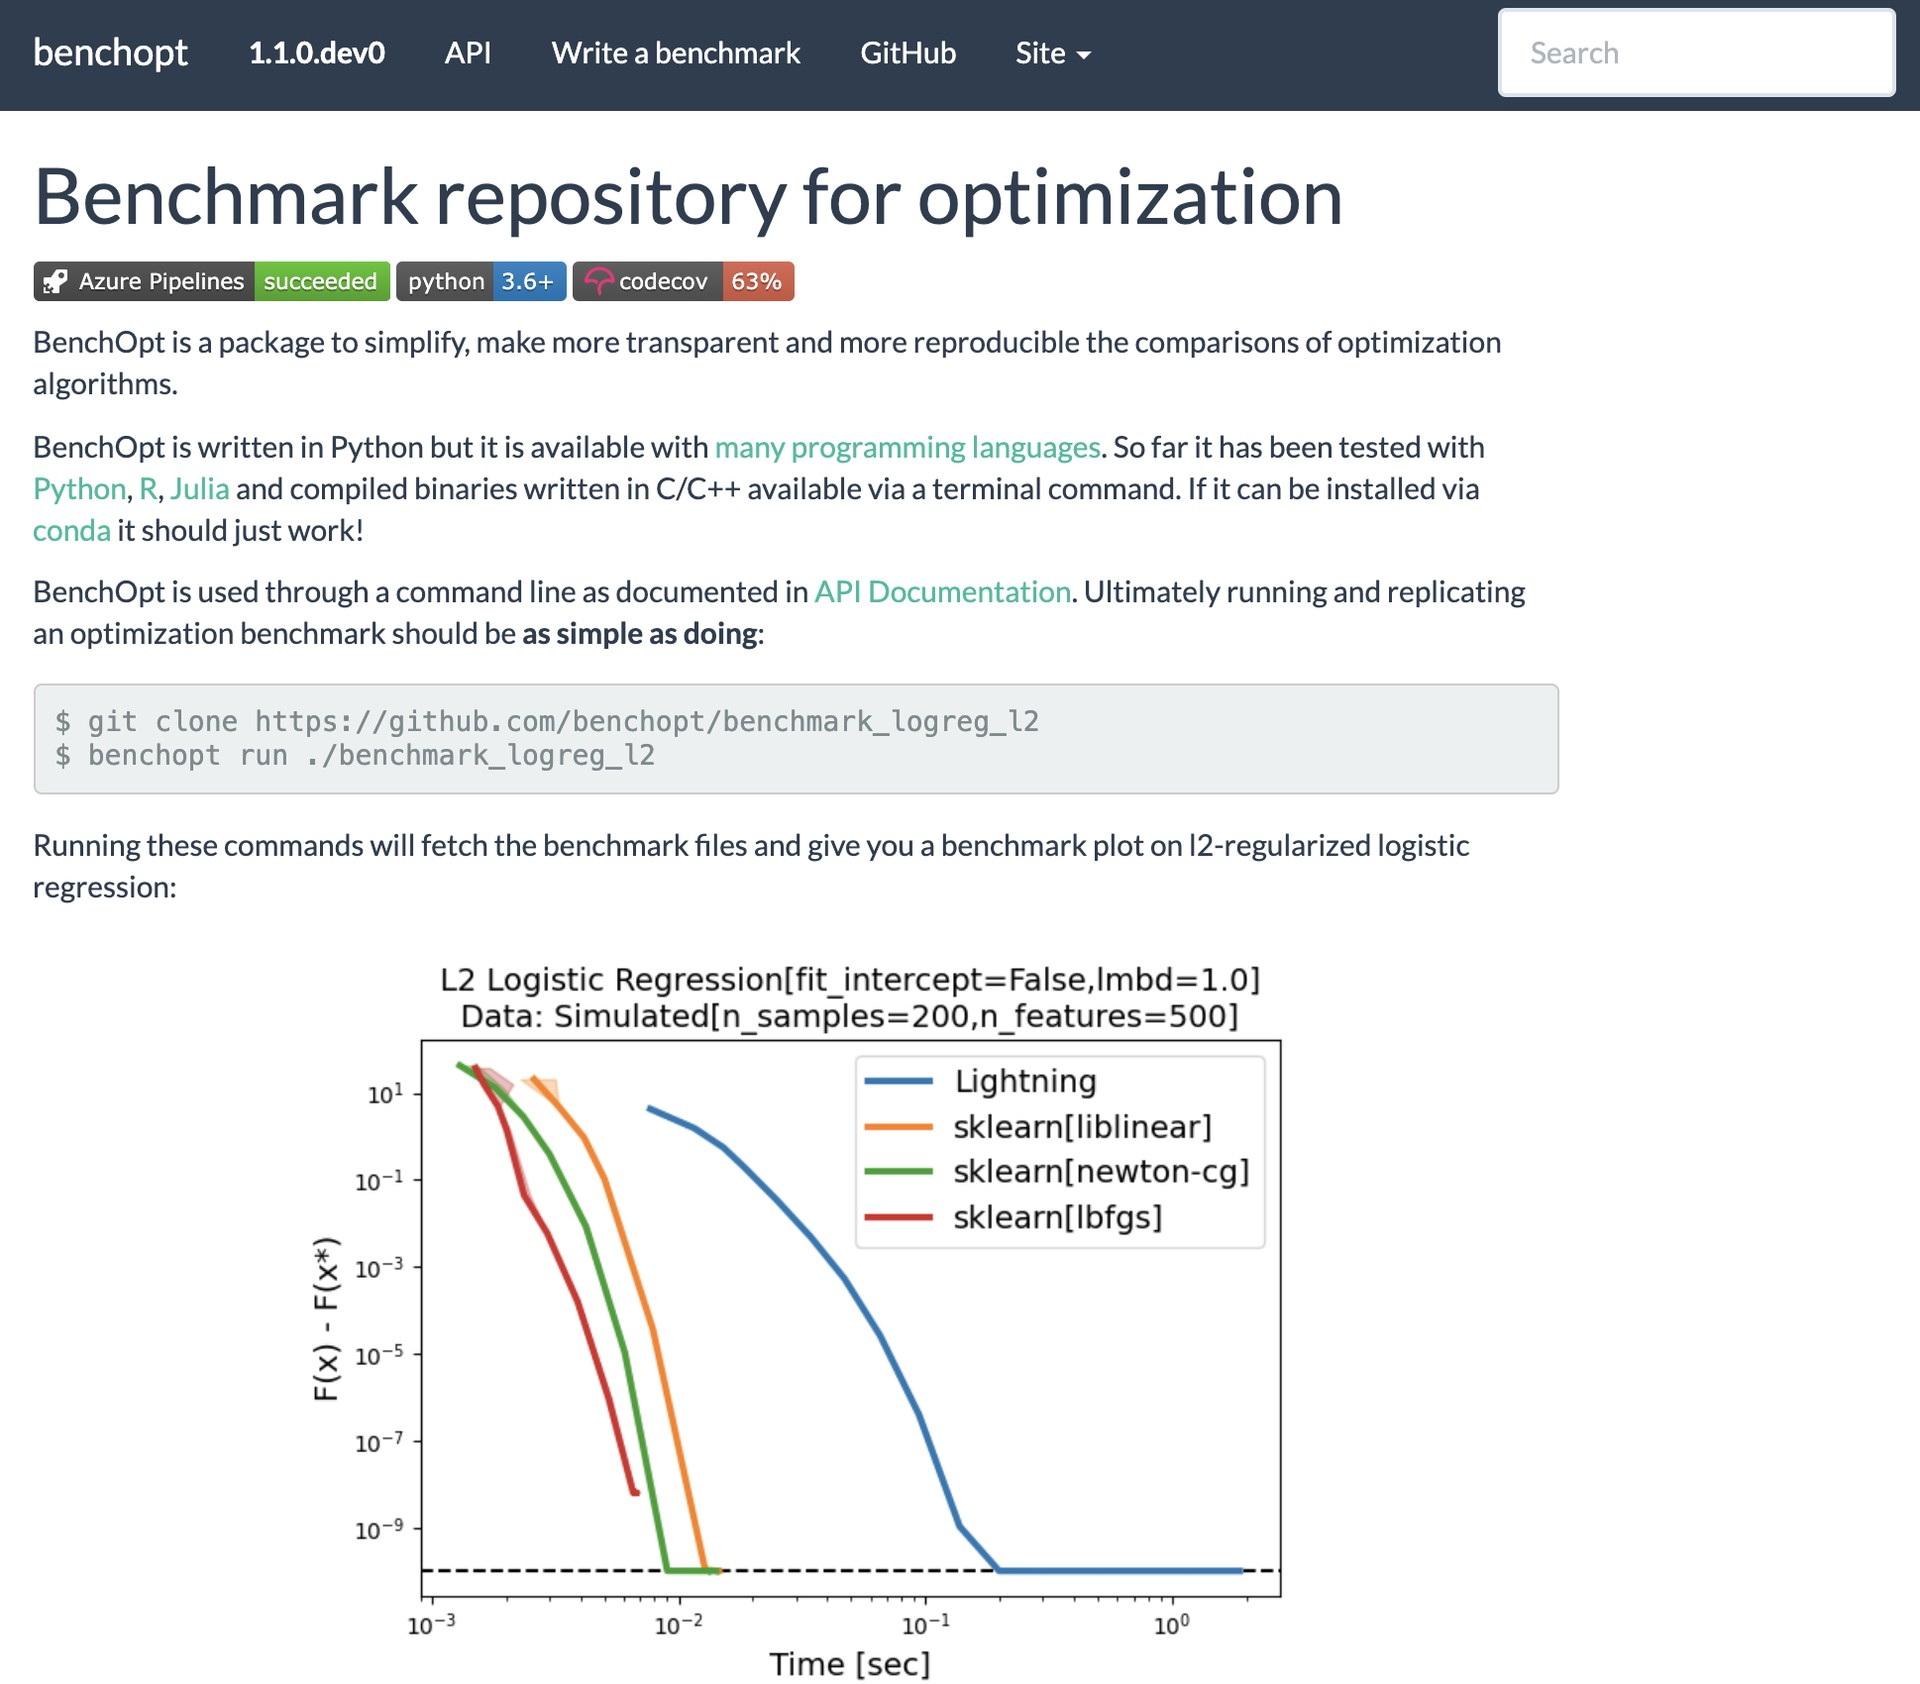
\includegraphics[width=.9\textwidth]{benchopt}\\
    }

\end{document}